%%%%%%%%%%%%湖南大学%%%%%%%%%%%%%%
%这里是湖南大学课程设计\LaTeX模板,版本1.0,适用于老师可接受PDF格式的论文,字体大小及样式可自行修改!
%请使用texlive 2020及以上版本使用xelatex引擎编译此模板!
%使用本模板出现的课程打分问题本人概不负责!
%欢迎各位使用本模板的同学与我多多交流,E-mail:hnuzyx@outlook.com
%%%%%%%%%%%%湖南大学%%%%%%%%%%%%%%
\documentclass{hnureport}

%-------------------------------------------------------------
\usepackage{enumitem,fancyvrb}
\usepackage{booktabs,multirow,longtable,makecell} % 表格相关
\usepackage[final]{pdfpages} % 包含整页 pdf
\usepackage{float}
\usepackage{array}
%% 封面和相关表格


\renewcommand{\abstractname}{\large 摘要\\}%重定义摘要二字的大小
%\usepackage[backend=bibtex]{biblatex}
\usepackage[backend=biber,style=gb7714-2015]{biblatex}

\bibliography{ref}

\begin{document}
%% word版,填写1-4页,转为pdf,命名为’MB202206.pdf‘,放于当前路径
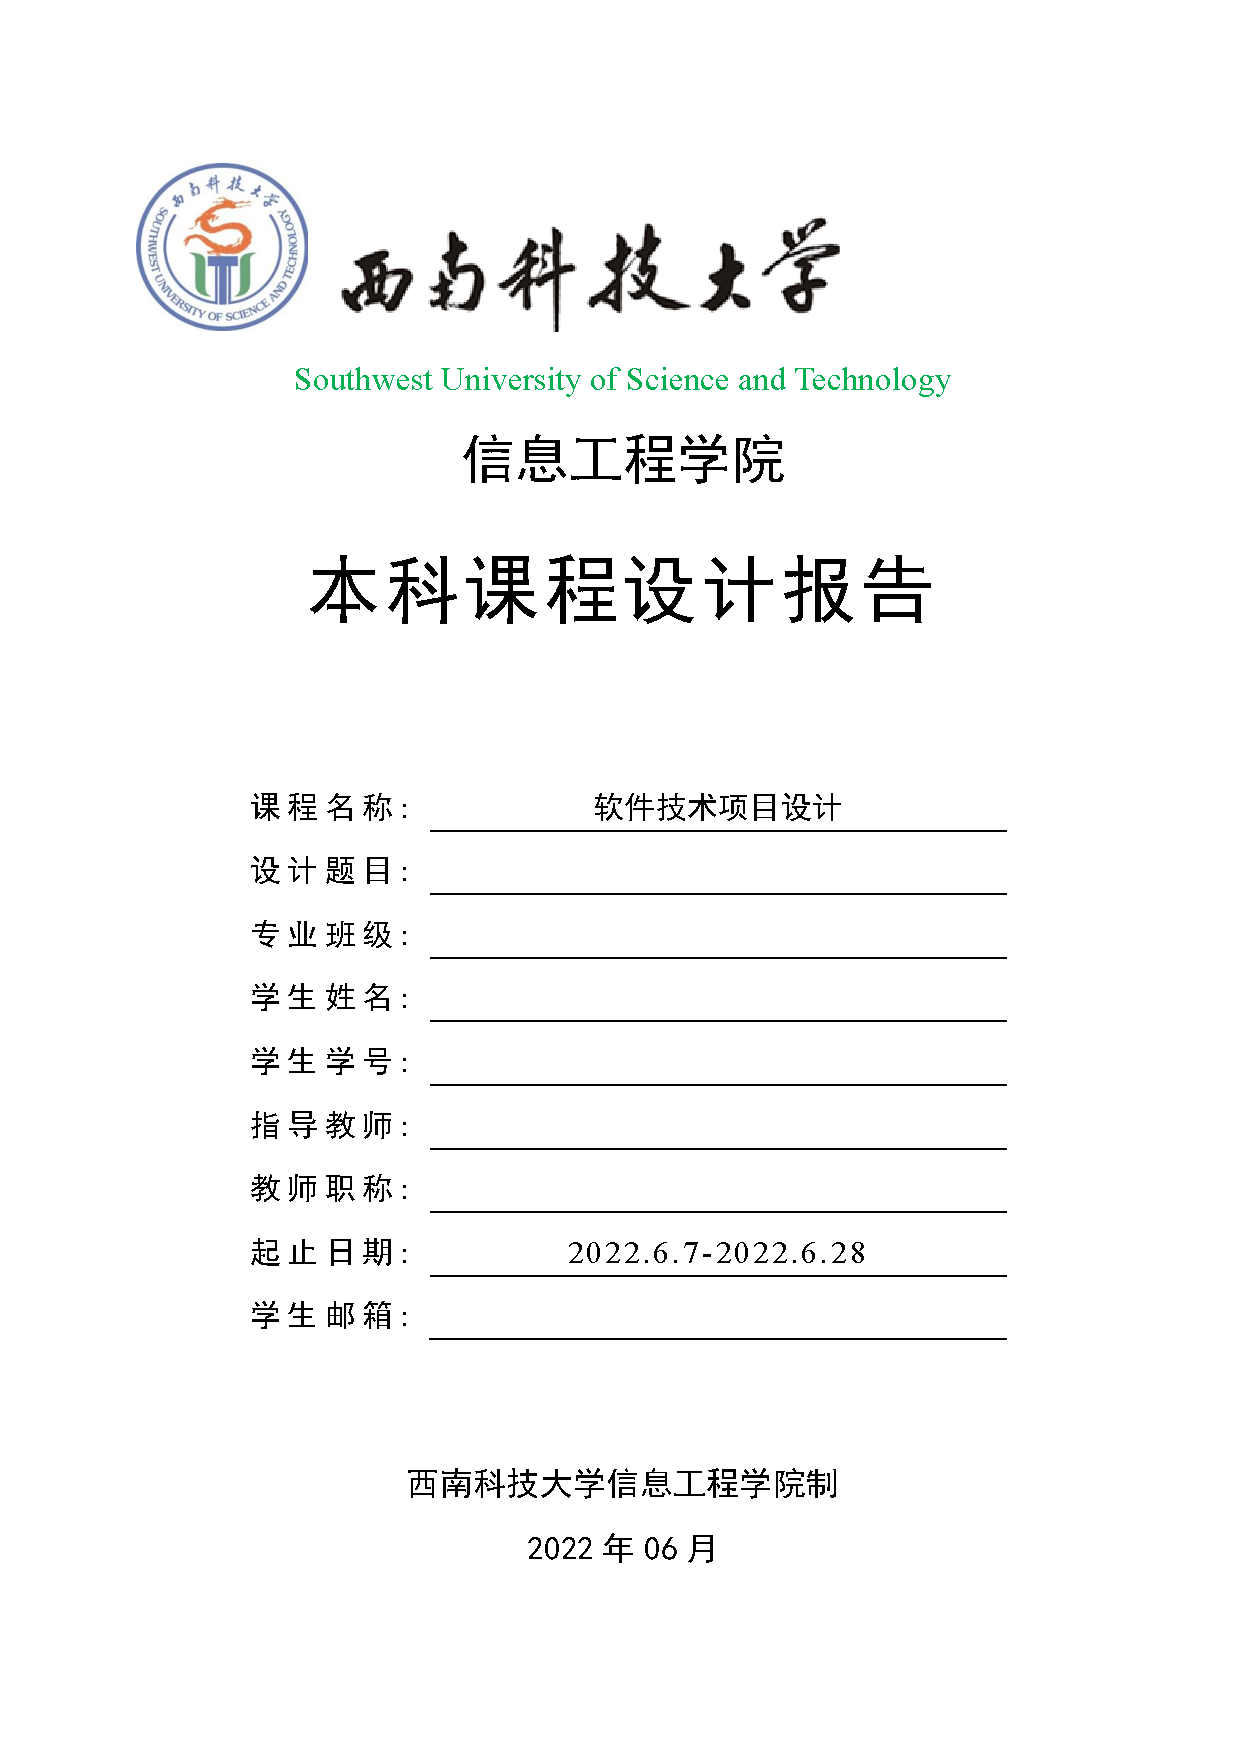
\includepdf[pages={1-4}]{MB202206.pdf}

% 生成题目
\begin{center}
\huge{\textbf{一个设计题目}}
\end{center}

\thispagestyle{empty}
\begin{abstract}
湖南大学(Hunan  University),简称“湖大”,坐落于长沙市,是教育部直属全国重点大学,教育部、工业和信息化部、湖南省人民政府、国家国防科技工业局共建高校,位列国家“世界一流大学建设高校”、“985工程”、“211工程”,入选国家“2011计划”、“111计划”、卓越法律人才教育培养计划、卓越工程师教育培养计划、国家建设高水平大学公派研究生项目、新工科研究与实践项目、全国深化创新创业教育改革示范高校、全国创新创业典型经验高校、全国高校实践育人创新创业基地、中国政府奖学金来华留学生接收院校、国家大学生创新性实验计划,高校国家知识产权信息服务中心。
 
湖南大学办学起源于公元976年创建的岳麓书院,历经宋、元、明、清等朝代的变迁,1897年创办新式高等学校时务学堂,1903年岳麓书院等合并改制为湖南高等学堂。1912年成立湖南高等师范学校。1926年成立省立湖南大学。1937年成为国民政府教育部16所国立大学之一.1949年9月,国立湖南大学更名为湖南大学。1950年8月20日,毛泽东同志亲笔题写校名。2000年,湖南大学与湖南财经学院合并组建成新的湖南大学。 

学校占地面积240万平方米,建筑面积145万平方米;设有研究生院和25个学院;本科招生专业63个;拥有一级学科博士点28个、专业学位博士点3个、一级学科硕士点35个、专业学位硕士点26个;建有国家重点学科一级学科2个、国家重点学科二级学科14个、博士后科研流动站28个;有教职工近4000人,有全日制在校学生36000余人。
\end{abstract}

\noindent\textbf{关键词:} 湖南大学 \quad 千年学府 \quad 岳麓书院 \quad \LaTeX
\newpage%摘要

\thispagestyle{empty}
\tableofcontents
\newpage
\setcounter{page}{1}
%% 正文开始----------------------------------------------------
\section{课题重述与背景}
\subsection{课题重述}

机器学习\cite{qiu2020nndl}

深度学习\cite{LeCun2015deep}

HOG\cite{dalal2005histograms}

湖南大学电气与信息工程学院,起源可追溯到1921年湖南公立工业专门学校的电机科。1926年湖南大学定名时,电机科改为电机系。1953年电机系被调整到华中工学院,1958年恢复。1980年电机系与电子工程系合并为电气工程系,1999年成立电气与信息工程学院。 该院有电气工程系、自动化系、电子信息工程系、仪器科学系、电工电子技术系和1个实验中心。全院教职工160多人,学院拥有全职院士1人(罗安),双聘院士1人,国家“百千万人才工程”第一、二层次人选2人(王耀南,李树涛),国家杰出青年科学基金获得者2人(曹一家、李树涛),教育部新世纪优秀人才8人。在籍研究生、本科生近3000人。
\subsection{课题背景}
湖南大学数学学院是湖南大学历史最悠久的院系之一,它源始于清末1908年湖南优级师范学堂(湖南大学的前身)设立的数学本科,从1924年的数理系、1933年的数学系、1959年的数学力学系、1985年的应用数学系,2000年的数学与计量经济学院到2019年的数学学院,已历经了近百年的变革与发展,硕果累累。学院下设应用数学、基础数学、信息与计算科学、概率统计、计量经济5个系,应用数学、运筹学与控制论和高等数学3个研究所,科学与工程计算实验室和资料室。学院拥有数学学科博士后科研流动站,应用数学、计算数学2个博士点,应用数学、基础数学、计算数学、概率统计、运筹学与控制论5个硕士点,数学与应用数学、信息与计算科学2个本科专业。其中,应用数学学科是湖南省“十五”重点建设学科,数学与应用数学专业是湖南省重点专业,《高等数学》课程是国家级精品课程。

\clearpage


\section{课题结果}
学院院长为王耀南教授,曹一家教授为学校现任副校长,王耀南、罗安2位教授为“长沙市十大知识产权创造导师”。
学院科研基础好、学科综合优势强,已形成电力系统自动化、电机传动、工业自动化、测控与仪器、电子信息与通信工程、智能控制与图象处理、新型输配电新技术、高电能质量输配电理论和技术、大规模集成电路故障诊断等特色和优势研究方向。学院先后承担了国家 “九五”、“十五” 、“十一五”攻关项目,国家 “863”、国际合作重点项目,国家自然科学基金,国家创新基金,博士点基金和部省科研基金项目300多项,其他横向科研课题350余项,国家发明特等奖1项,国家科技发明三等奖1项,部、省科技进步一、二等奖和其他奖项120余项。07年到帐科研经费1500多万元。近年来国家科技进步二等奖有:王耀南4项:智能图像信息处理方法及其在工业系统中的应用;高速灌装生产线智能检测分拣成套装备研制及其推广应用等。罗安2项:电能质量先进控制方法及工程应用;大型企业综合电气节能关键技术及应用;国家技术发明二等奖有:罗安一项:冶金特种大功率电源系统关键技术与装备及其应用。近2年获得IEEE第三大区唯一杰出工程师年度大奖1人,全国优秀科技工作者1人。

电气与信息工程学院传承“爱国务实、经世致用”的优良传统,积极参与“推进富民强省、争当五一先锋”竞赛,在教学、科研、学科建设等领域喜获全面丰收。一是人才培养卓有成效。学院确立人才培养的中心地位,创新人才培养成绩突出,近三年指导博士生获,“全国百篇优秀博士学位论文”获得者1人,省优秀博士论文5篇、省优秀硕士论文12篇、在全国“挑战杯” 大学生创业大赛上荣获金奖3人、全国大学生智能车竞赛上荣获一等奖6项;教学研究和教学改革成果显著,先后承担国家级教改项目1项、省部级教改项目5项。获国家级教学成果二等奖1项,省级教学成果一等奖1项,二等奖3项;工业自动化专业被评为国家特色专业,电气工程及其自动化专业被列为湖南省重点专业。二是科学研究硕果累累。学院围绕国家经济和国防建设重大需求,集中力量,以国家 “973”项目、“863”计划、国家重大科技专项、国家科技支撑计划、国家自然基金重点项目、湖南省重大专项为突破口,积极服务于国家和地方经济,实现了产学研的有机结合。形成了多个高水平科研团队,营造了良好的科研环境。近三年新增科研项目170项,科研项目到帐总经费8274万元,出版教材、学术专著15部,获得发明专利47项、软件著作权51项、实用新型专利33项,学术论文被三大检索收录479篇,荣获各类科技奖励共34项,其中国家科技进步二等奖4项,省部级奖励19项。三是学科建设成绩突出。学院已拥有十分完备的学科体系,拥有“控制理论与控制工程”国家重点学科,“电工理论与新技术”国家重点培育学科;拥有1个机器人感知与控制技术国家工程实验室,1个电能变换与控制国家工程技术研究中心,1个电力驱动与伺服技术国防重点学科实验室,2个教育部工程研究中心,1个教育部重点实验室,1个国防技术重点实验室,2个湖南省重点实验室,2个机械工业联合会重点实验室,2个博士后科研流动站,2个一级学科博士点,11个二级学科博士点,17个硕士点。四是综合管理井然有序。学院形成了“拼搏、奉献、和谐、快乐”的学院文化,制度健全、管理完善,院务公开、民主决策、勤政廉政,注重依靠教职工共商发展大计,凝心聚力,有关学院建设和发展的重大决策和涉及教职工切身利益的重大事项,都必须通过教职工代表大会的民主决策。学院呈现出持续快速发展的良好局面,党建与思政工作连续六年被评为学校优秀单位;部门工会连续七年被评为先进集体,2010年被授予湖南大学先进教职工之家称号,2011年被湖南省总工会授予“湖南省五一先锋集体”荣誉称号,2010年湖南省教育系统唯一获得该项荣誉的单位。

\clearpage



% \section*{参考文献}
\printbibliography
\clearpage

\appendix

\newpage
\section{附录一:matlab代码}
\begin{lstlisting}[language=matlab]
[X, Y] = meshgrid(0.01:0.01:1, 0.01:0.01:1); 
Zfun =@(x,y)12.5*x.*log10(x).*y.*(y-1)+exp(-((25 ... 
*x - 25/exp(1)).^2+(25*y-25/2).^2).^3)./25; 
Z = Zfun(X,Y); 
figure; 
surf(Y,Z,X,'FaceColor',[1 0.75 0.65],'linestyle','none'); 
hold on 
surf(Y+0.98,Z,X,'FaceColor',[1 0.75 0.65],'linestyle','none'); 
axis equal; 
view([116 30]); 
camlight; 
lighting phong; % 设置光照和光照模式
\end{lstlisting}

\section{附录二:python代码}
\begin{lstlisting}[language=python]
def run():
from sko.GA import GA_TSP
import numpy as np
from scipy import spatial
from numpy.linalg import norm
import cvxpy as cp
import pandas as pd 
#python原始代码
data=pd.read_excel("3.xlsx")
\end{lstlisting}


\end{document}
